\documentclass[pdflatex,11pt]{../aghdoc}
%\documentclass{../aghdoc}               % przy kompilacji programem latex
\usepackage[polish]{babel}
\usepackage[utf8]{inputenc}

% dodatkowe pakiety
\usepackage{hyperref}
\usepackage{enumerate}
\usepackage{listings}
\lstloadlanguages{TeX}

\lstset{
  literate={ą}{{\k{a}}}1
           {ć}{{\'c}}1
           {ę}{{\k{e}}}1
           {ó}{{\'o}}1
           {ń}{{\'n}}1
           {ł}{{\l{}}}1
           {ś}{{\'s}}1
           {ź}{{\'z}}1
           {ż}{{\.z}}1
           {Ą}{{\k{A}}}1
           {Ć}{{\'C}}1
           {Ę}{{\k{E}}}1
           {Ó}{{\'O}}1
           {Ń}{{\'N}}1
           {Ł}{{\L{}}}1
           {Ś}{{\'S}}1
           {Ź}{{\'Z}}1
           {Ż}{{\.Z}}1
}

%---------------------------------------------------------------------------

\author{Tomasz Kasprzyk, Daniel Ogiela, Jakub Stępak}
\shortauthor{T. Kasprzyk, D. Ogiela, J.Stępak}

\titlePL{System obliczający wyniki wyborów dla uogólnienia systemu k-Borda}

\shorttitlePL{System obliczający wyniki wyborów dla uogólnienia systemu k-Borda} % skrócona wersja tytułu jeśli jest bardzo długi

\thesistypePL{Dokumentacja użytkownika}

\supervisorPL{dr hab. inż. Piotr Faliszewski}

\date{2016}

\departmentPL{Katedra Informatyki}

\facultyPL{Wydział Informatyki, Elektroniki i Telekomunikacji}

\setlength{\cftsecnumwidth}{10mm}

%---------------------------------------------------------------------------

\begin{document}

\titlepages

\tableofcontents


%----------------------------------------------------------------------------
\chapter{Wstęp}
\label{cha:wstep}

Niniejszy podręcznik opisuje sposób użytkowania systemu \texttt{Election Computing System}, powstałego w ramach pracy inżynierskiej realizowanej na Akademii Górniczo-Hutniczej w Krakowie.

System umożliwia obliczenie wyników wyborów w uogólnionym systemie wyborczym k-Borda. Szczegóły na temat tego systemu wyborczego można przeczytać w Przewodniku po projekcie.


\chapter{Instrukcja uruchomienia systemu}
\label{cha:uruchomienie}

Działającą aplikację można przetestować na stronie: \\ \url{https://election-computing-system.herokuapp.com}. 

Ze względu na ograniczenia na ilość rekordów w bazie danych narzucone przez darmową wersję Heroku, nie będzie można dodać tam zbyt „dużych” wyborów (ograniczona jest liczba głosujących i kandydatów). Aby korzystać z pełnych możliwości aplikacji, należy uruchomić ją na własnym komputerze. Dalsza część tego rozdziału opisuje jak to wykonać.

\section{Przygotowanie środowiska}
\label{sec:srodowisko}

\subsection{Język}
\label{subsec:jezyk}

System jest aplikacją internetową opartą o framework Django napisaną w języku Python 2.7.
Aby uruchomić aplikację, należy uprzednio zainstalować na swoim komputerze interpreter Pythona.

\subsection{Repozytorium}
\label{subsec:repo}

Repozytorium projektu znajduje się pod adresem: \\ \url{https://github.com/jakubste/election-computing-system}.
Projekt należy sklonować używając programu Git 
\begin{lstlisting}[language=bash]
$ git clone git@github.com:jakubste/election-computing-system.git
\end{lstlisting}
lub ściągnąć jako ZIP bezpośrednio z GitHuba i rozpakować w wybranym miejscu.

\subsection{Biblioteki}
\label{subsec:biblioteki}

Do instalacji bibliotek zaleca się używanie mechanizmu \texttt{virtualenv}, który separuje środowiska uruchomieniowe dla poszczególnych projektów. Autorzy projektu zalecają też dla wygody wykorzystanie \texttt{virtualenvwrapper}'a. Do instalacji bibliotek można użyć programu \texttt{pip}.
Informacje o wymaganych bibliotekach są zawarte w pliku \texttt{requirements.txt}.
\begin{lstlisting}[language=bash]
$ mkvirtualenv inz
$ pip install -r requirements.txt
\end{lstlisting}

\subsection{Baza danych}
\label{subsec:database}

Aplikacja domyślnie jest skonfigurowana do użycia z bazą danych dostarczaną przez Heroku (PostreSQL). Dla ułatwienia zostanie przedstawiony sposób konfiguracji z użyciem SQLite3. O konfiguracji dostępu do innych baz danych można przeczytać w dokumentacji Django. 

W celu skonfigurowania swojej bazy danych należy w katalogu \texttt{ecs} utworzyć 
plik \texttt{local\_settings.py} i umieścić tam następujący kod:

\begin{lstlisting}[language=Python]
from settings import *

DATABASES = {
   'default': {
       'ENGINE': 'django.db.backends.sqlite3',
       'NAME': os.path.join(BASE_DIR, 'db.sqlite3'),
   }
}
\end{lstlisting}

Następnie w katalogu głównym programu należy wykonać polecenie:
\begin{lstlisting}[language=bash]
$ ./manage.py migrate
\end{lstlisting}


\section{Uruchomienie serwera}
\label{sec:serwer}

W tym momencie aplikacja powinna być gotowa do działania.
W katalogu głównym programu należy wykonać polecenie:
\begin{lstlisting}[language=bash]
$ ./manage.py run_server
\end{lstlisting}

Po otworzeniu w przeglądarce internetowej adresu:
\begin{lstlisting}
http://localhost:8000/
\end{lstlisting}
powinna pojawić się strona podobna do tej:


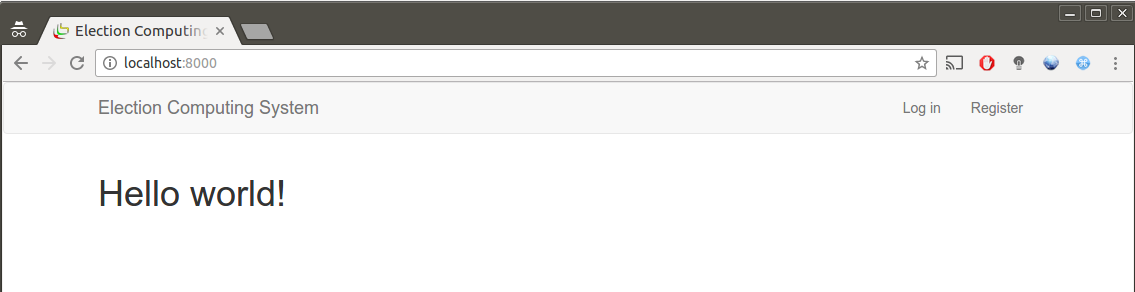
\includegraphics[width=0.8\textwidth]{pics/first_view.png}


\chapter{Instrukcja obsługi systemu}
\label{cha:obsluga}


\section{Rejestracja}
\label{sec:rejestracja}

Aby korzystać z systemu, należy utworzyć konto. W tym celu należy z menu wybrać opcję rejestracji i uzupełnić formularz:

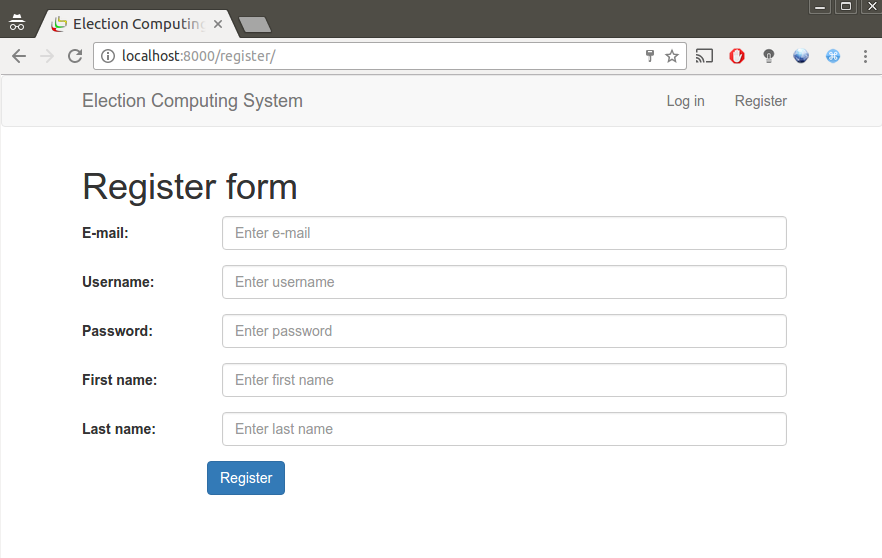
\includegraphics[width=0.8\textwidth]{pics/register.png}

\newpage
\section{Logowanie}
\label{sec:logowanie}

W celu zalogowania się na wcześniej utworzone konto należy wybrać z menu opcję logowania i wypełnić formularz:

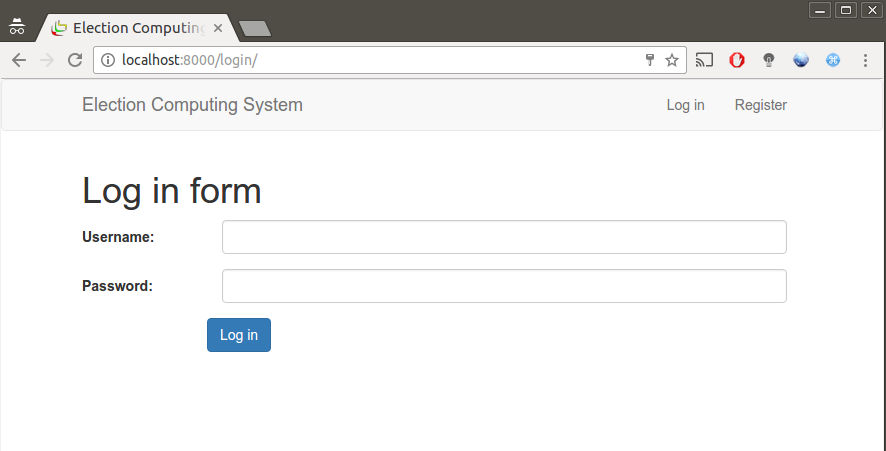
\includegraphics[width=0.8\textwidth]{pics/login.png}


\section{Strona główna}
\label{sec:stronaglowna}

Po zalogowaniu użytkownik widzi stronę główną z opisem systemu:

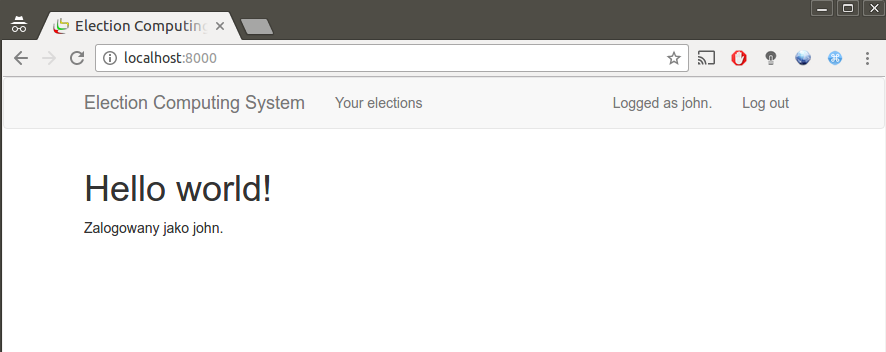
\includegraphics[width=0.8\textwidth]{pics/mainpage.png}


\newpage
\section{Lista wyborów}
\label{sec:electionslist}

Po wybraniu z menu listy wyborów użytkownik ma możliwość zobaczenia listy swoich wyborów:

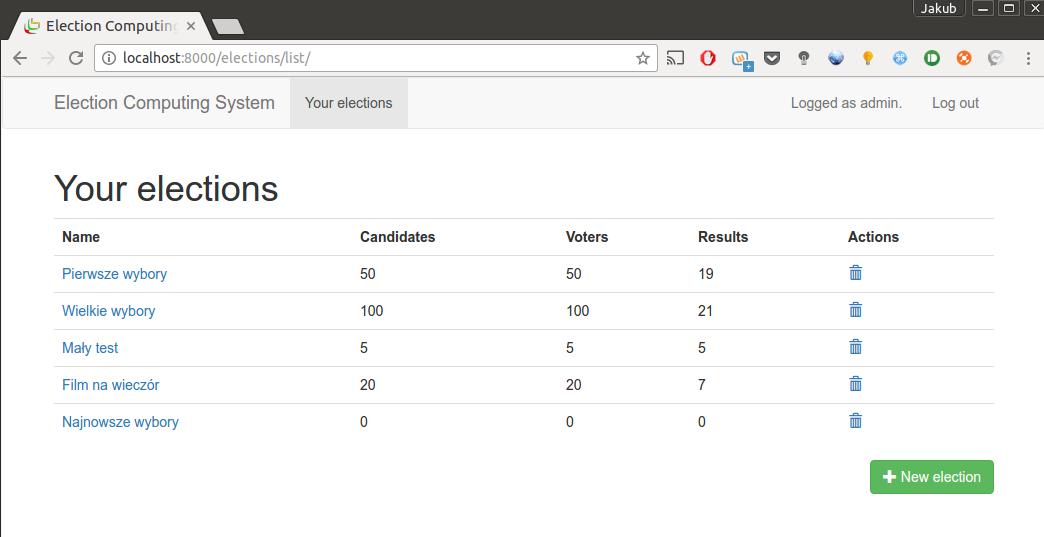
\includegraphics[width=0.8\textwidth]{pics/elections-list.png}

Stąd użytkownik ma możliwość przejścia do tworzenia nowych wyborów.


\section{Tworzenie wyborów}
\label{sec:electionscreate}

Aby utworzyć nowe wybory należy podać ich nazwę oraz określić rozmiar komitetu do którego przeprowadzamy wybory:

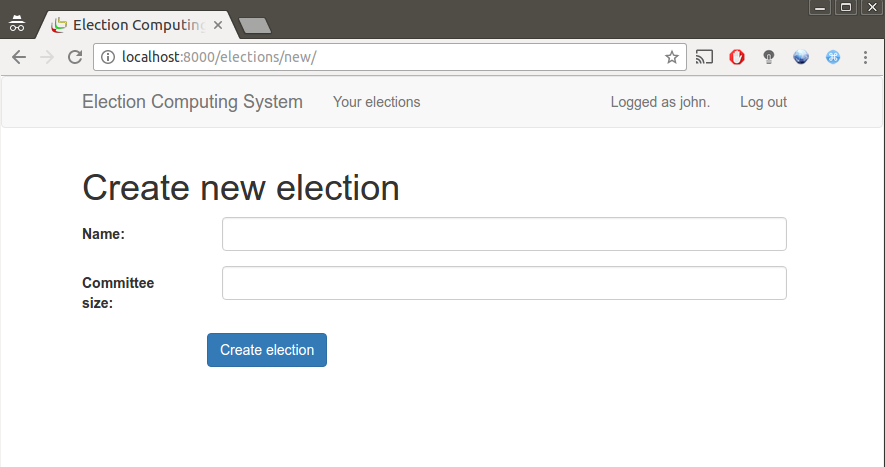
\includegraphics[width=0.8\textwidth]{pics/elections-new.png}

\newpage
\section{Określenie kandydatów i wyborców}
\label{sec:electionsnewlycreated}

Po utworzeniu wyborów należy określić biorących udział w wyborach kandydatów oraz wyborców.

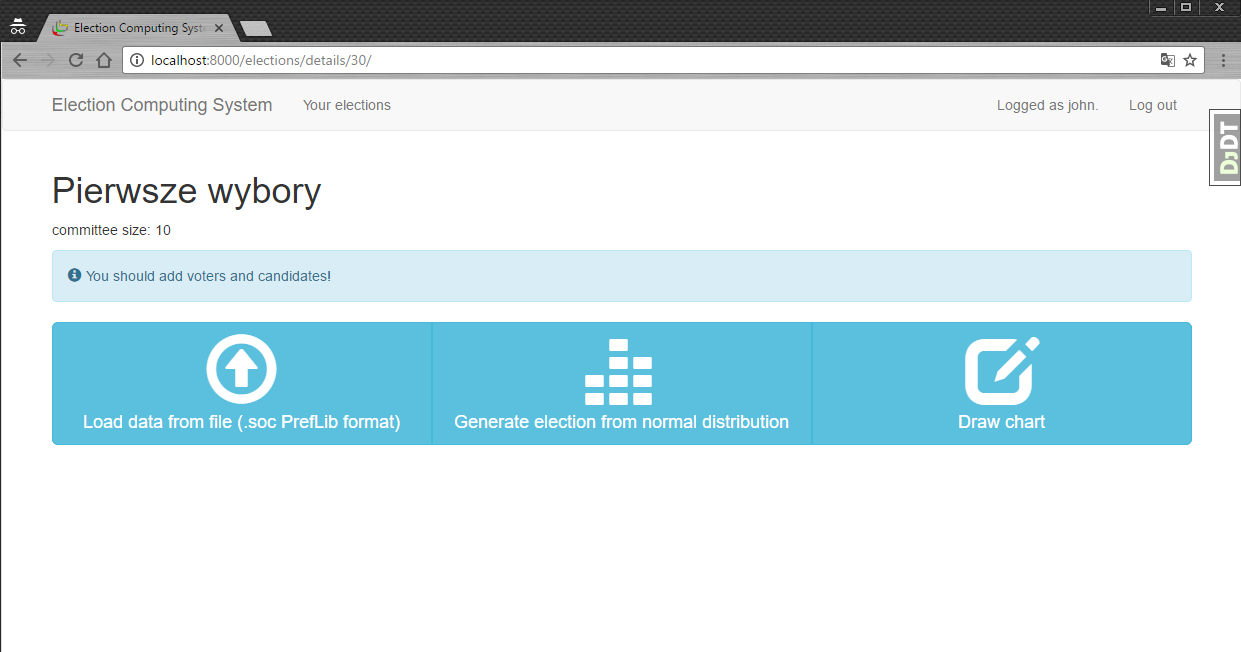
\includegraphics[width=0.8\textwidth]{pics/elections-config.png}

Użytkownik ma do wyboru dwie opcje:
\begin{itemize}
\item wczytać dane z pliku w formacie .soc określonym przez \href{http://www.preflib.org/}{PrefLib},
\item wygenerować losowy układ wyborców w oparciu o rozkład naturalny.
\end{itemize}


\subsection{Wczytanie danych z pliku}
\label{subsec:wczytaniezpliku}

Aby wczytać dane dotyczące wyborów z pliku należy wybrać odpowiednią opcję a następnie wskazać plik z danymi:

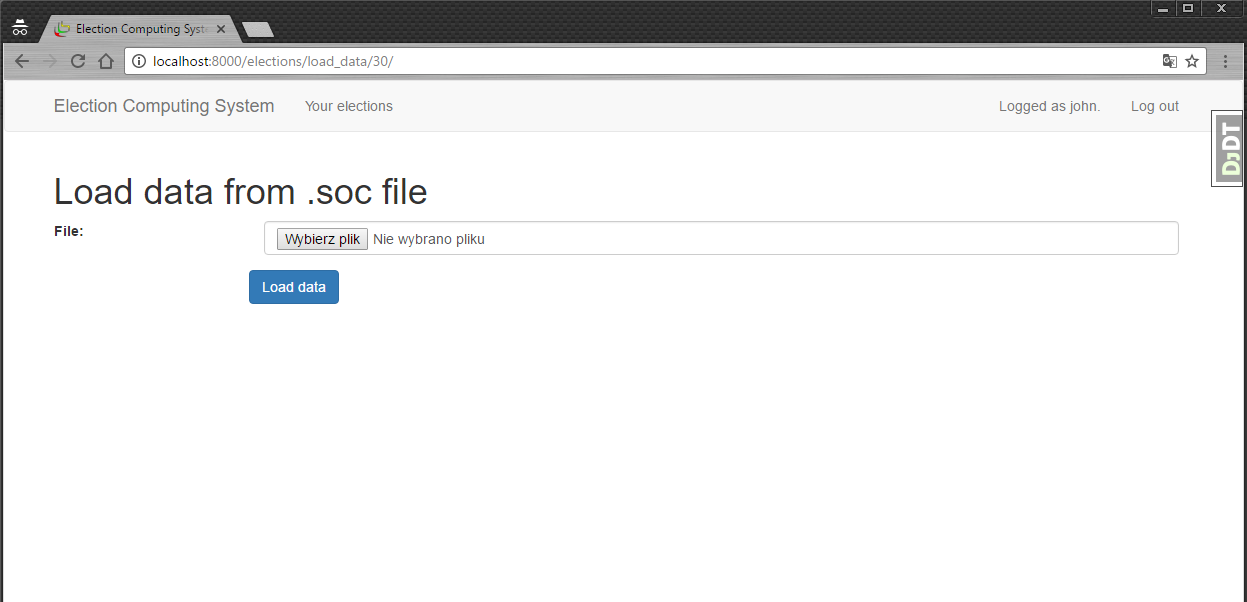
\includegraphics[width=0.8\textwidth]{pics/load-from-file.png}

Przykładowe pliki z danymi można pobrać ze strony projektu \href{http://www.preflib.org/data/packs/index.php#soc}{PrefLib}. Pośród tych plików można m.in. znaleźć rzeczywiste preferencje studentów naszego kierunku w wyborach przedmiotów obieralnych.

\newpage
\subsection{Generacja danych z rozkładu normalnego}
\label{subsec:generowaniedanych}

Aby wygenerować dane losowe na podstawie rozkładu normalnego należy wybrać odpowiednią opcję, a następnie uzupełnić formularz:
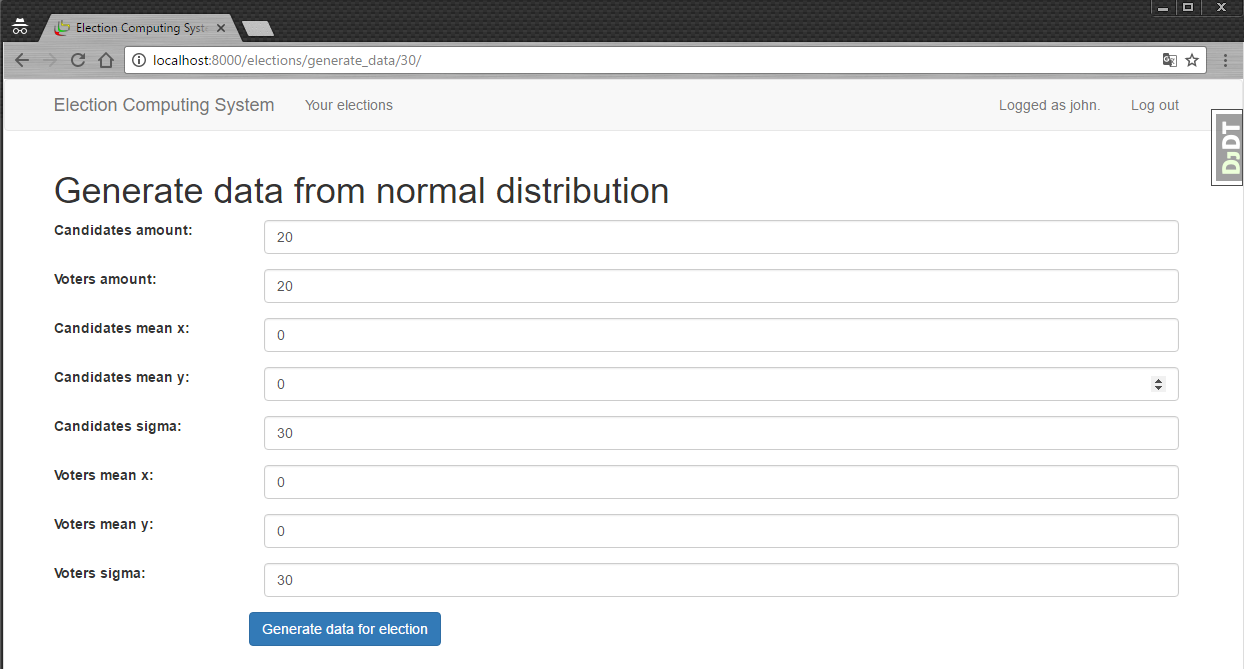
\includegraphics[width=0.8\textwidth]{pics/generate-distribution.png}

W formularzu należy określić liczbę kandydatów i głosujących, punkt centralny, wokół którego będą skupione ich „poglądy” oraz sigmę, czyli średni „rozstrzał” poglądów.

Koncepcyjnie ten sposób generacji danych odzwierciedla mapę poglądów politycznych. Porządek preferencji kandydatów wśród wyborców określa ich odległość euklidesowa w układzie współrzędnych.

W dalszej części instrukcji będziemy posługiwali się częściej przykładem z wyborami wygenerowanymi w ten sposób.


\section{Szczegóły wyborów}
\label{sec:szczegolywyborow}

Po wczytaniu danych pokaże się ekran z szczegółami wyborów:
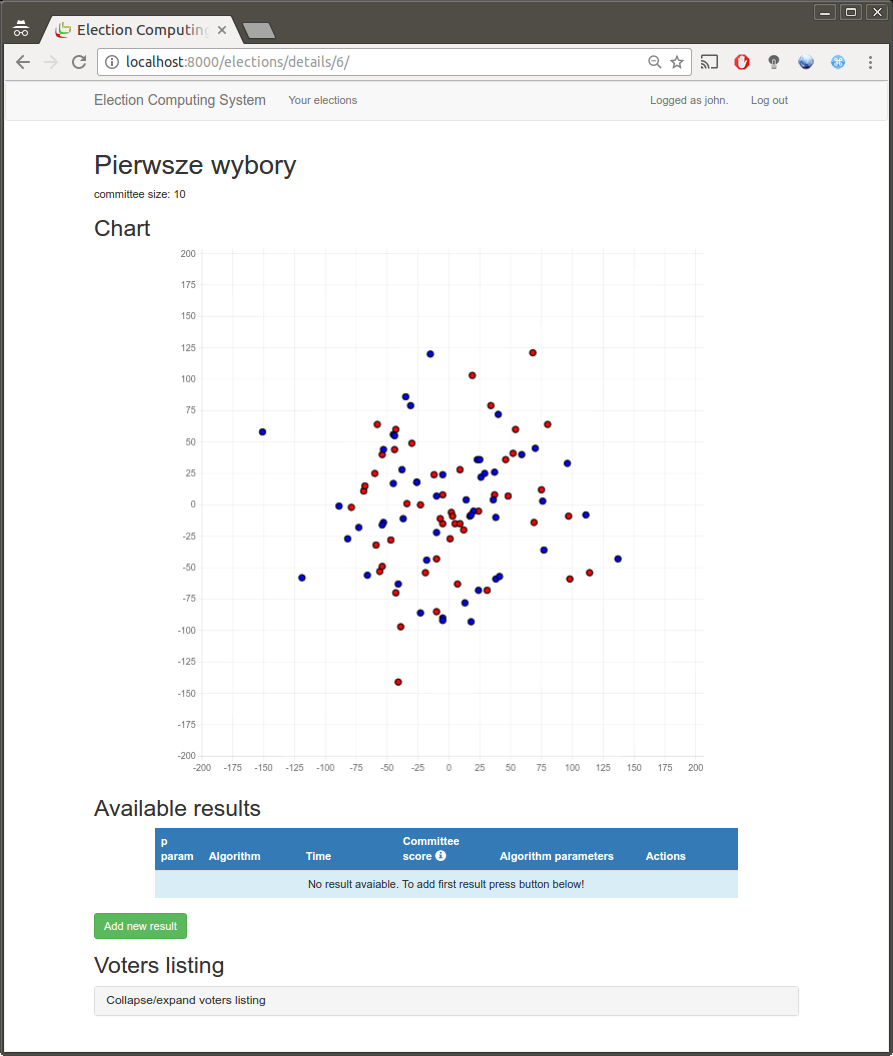
\includegraphics[width=0.8\textwidth]{pics/newlycreated.png}

Wykres będzie widoczny tylko w przypadku wyborów wygenerowanych z rozkładu normalnego.

Poniżej można zobaczyć spis dostępnych rozstrzygnięć wyborów oraz odnośnik do formularza dodawania nowego wyniku.

Poniżej, jeśli liczba wyborców nie jest na tyle duża, że utrudniałoby to używanie strony przez zbytnie obciążenie przeglądarki, widać listing wyborców. Szczególnie przydatny do sprawdzenia czy poprawnie zostały wczytane dane z plików .soc. W przypadku danych z rozkładu normalnego jego przydatność jest ograniczona.

\newpage
\section{Dodawanie wyniku}
\label{sec:dodawaniewyniku}


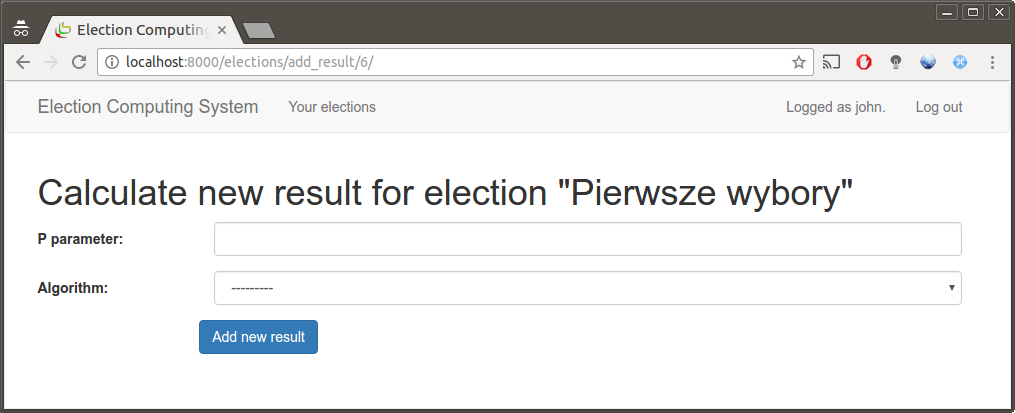
\includegraphics[width=0.8\textwidth]{pics/new-result.png}

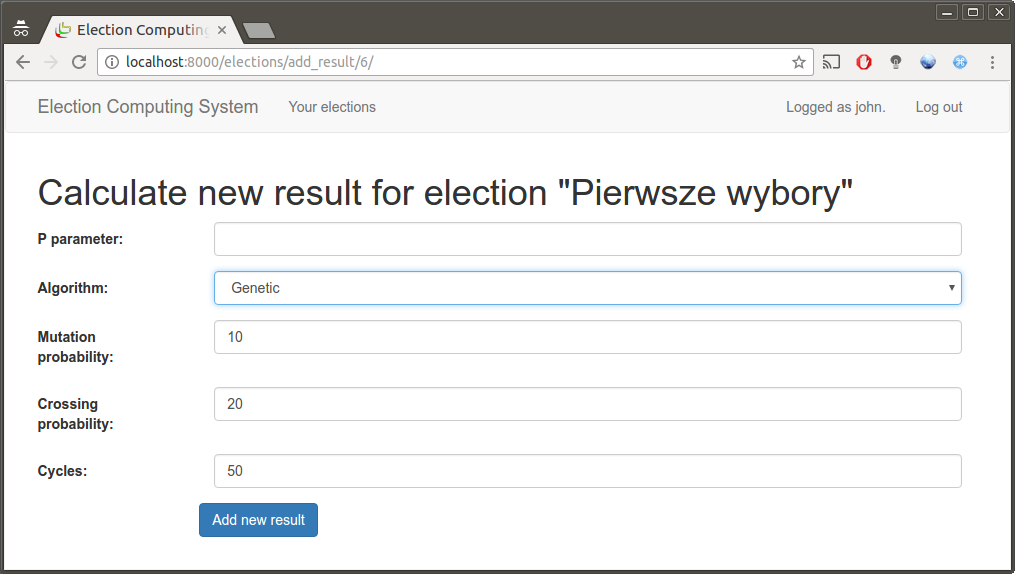
\includegraphics[width=0.8\textwidth]{pics/new-result-genetic.png}

\newpage
\section{Porównywanie wyników}
\label{sec:porownywaniewynikow}

\subsection{Używanie wykresu do porównywania wyników}
\label{subsec:pornawykresie}

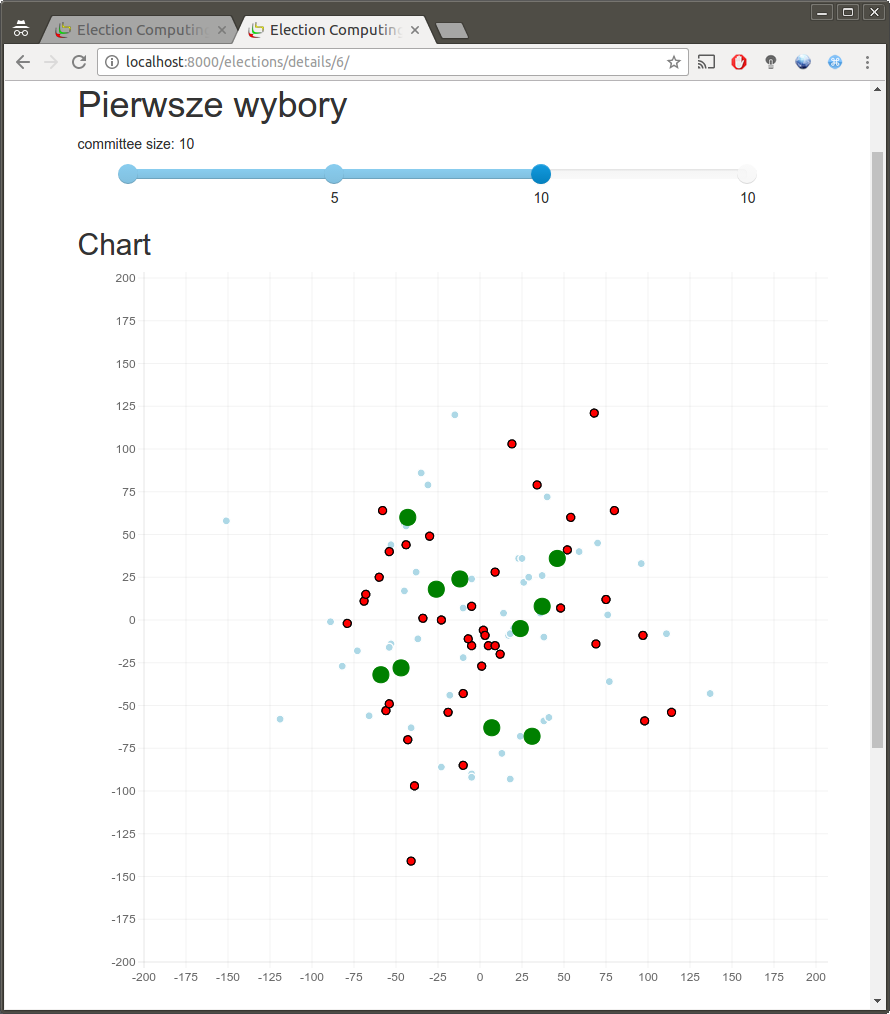
\includegraphics[width=0.8\textwidth]{pics/results-on-chart.png}

\newpage
\subsection{Zestawienie wyników w tabeli}
\label{subsec:tabelazwynikami}

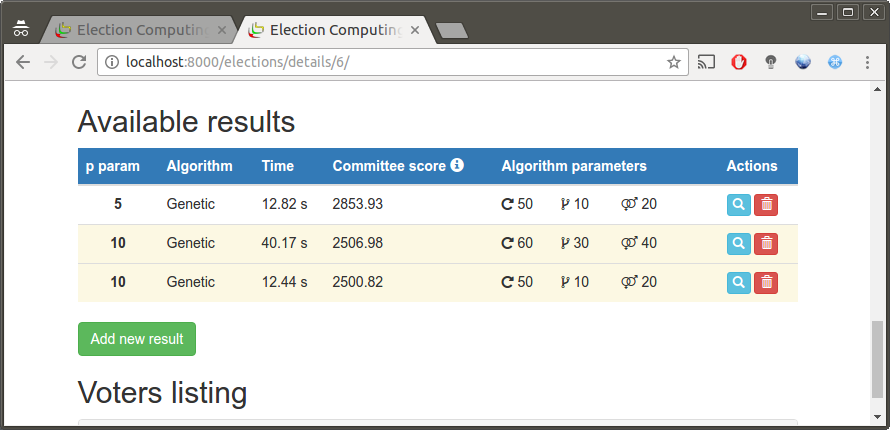
\includegraphics[width=0.8\textwidth]{pics/results-on-table.png}


\newpage
\section{Szczegóły wyniku}
\label{sec:szczegolywyniku}

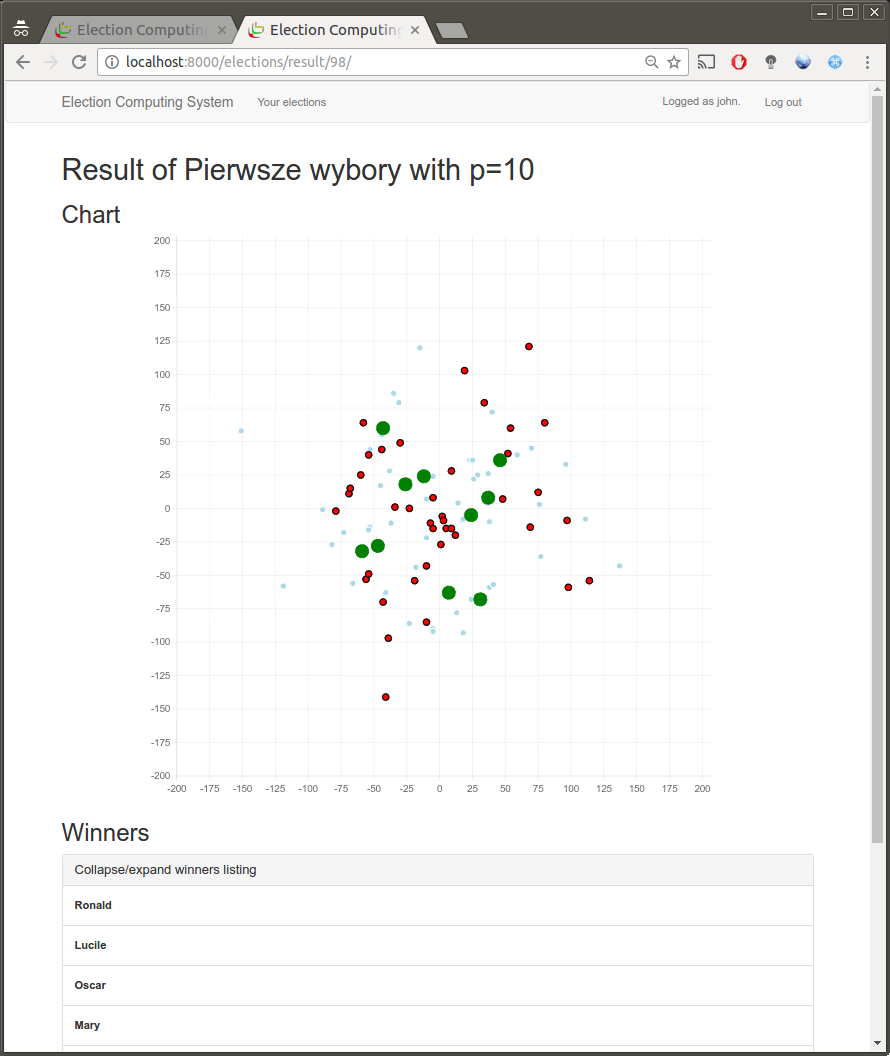
\includegraphics[width=0.8\textwidth]{pics/result-details.png}


\newpage
\section{Kasowanie wyników}
\label{sec:kasowaniewynikow}

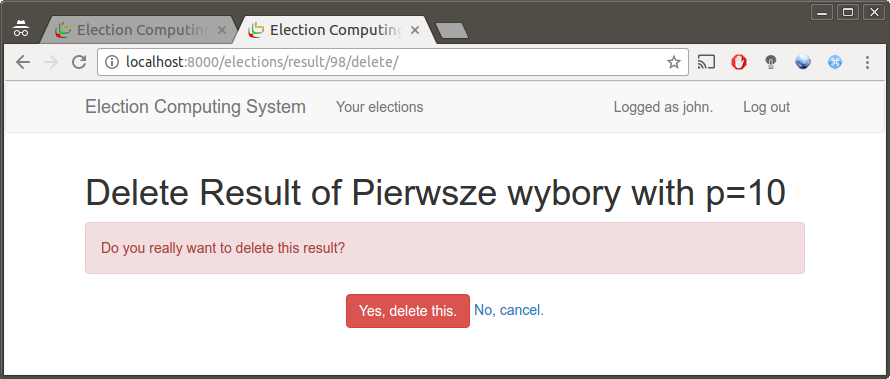
\includegraphics[width=0.8\textwidth]{pics/delete-result.png}


\section{Kasowanie wyborów}
\label{sec:kasowaniewyborow}

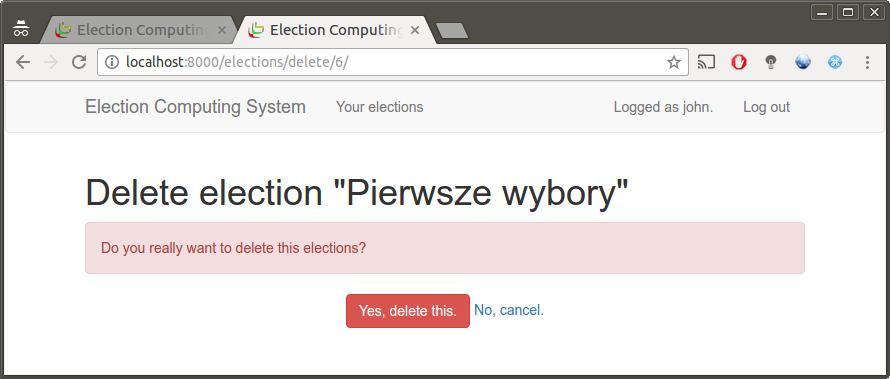
\includegraphics[width=0.8\textwidth]{pics/delete-elections.png}



\chapter{Podsumowanie}
\label{cha:podsumowanie}

Twórcy systemu dążyli do zapewnienia dwóch podstawowych dogodności dla użytkowników. Pierwszą z nich była przystępna forma prezentacji wyników a drugą intuicyjna nawigacja po stronie.

\section{Prezentacja wyników}
Odpowiednia forma prezentacji wyników była sprawą nieodzowną dla dobrego działania systemu. Poza wymiarem estetycznym umożliwia zaobserwowanie sposobu zmieniania się wyników wyborów w zależności od parametrów przekazanych algorytmowi. W celu udogodnienia porównywania różnych wyników wyborów zaimplementowano suwak, który pozwala na proste przechodzenie między kolejnymi wykresami. W trakcie przechodzenia między wykresami punkty nie zmieniają swojego położenia na ekranie, dlatego wyraźnie widać każdą zmianę pomiędzy danymi wynikami wyborów.
 
Innym udogodnieniem, które zostało wprowadzone jest sposób wyświetlania tabeli z czasami działania algorytmów oraz zadowoleniami jakie osiągnęły algorytmy. Poza estetyczną prezentacją tabeli, wyniki grupowane są według parametru p - wyniki dla tego samego parametru p są obok siebie. Ponadto tło grupy wyników jest pokolorowane w taki sposób, aby sąsiednie grupy miały inne tło. Dzięki takim zabiegom w prosty sposób można zlokalizować grupy wyników dla tego samego parametru p.

\section{Nawigacja po stronie}

Zarządzanie swoimi wyborami i ich wynikami było drugim aspektem, nad którym pochylili się twórcy aplikacji. Dążono do możliwie intuicyjnego interfejsu, który w łatwy sposób pozwoliłby na wykonywanie usług zapewnianych przez system. Przyciski zatwierdzające dane operacje odróżniają się od innych elementów strony przez co są łatwo widoczne. Ciąg operacji, które wykonuje użytkownik w celu wykonania danej akcji jest możliwie prosty i intuicyjny. Wyniki wyborów i same wybory są zgrupowane oddzielnie. Wyraźnie odróżnione są elementy klikalne i możliwe tylko do wyświetlenia.

\chapter{Spis rysunków}
\label{cha:rysunki}



\bibliographystyle{alpha}
\bibliography{bibliografia}

\end{document}
